\chapter{Special Functions}

%%%%%%%%%%%%%%%%%%%%%%%%%%%%%%%%%%%%%%%%%%%%%%%%%%%%%%%%%%%%
\section{Gamma Function}

%%%%%%%%%%%%%%%%%%%%%%%%%%%%
\begin{definition} \label{D:gamma}
The gamma function is defined by 
\begin{equation}
  \Gamma(z) = \int_0^{\infty} t^{z-1} e^{-t} dt.
\end{equation}
\end{definition}

%%%%%%%%%%%%%%%%%%%%%%%%%%%%
\begin{proposition} \label{P:gamma_pp}
The gamma function $\Gamma(z)$ has the following properties:
\begin{enumerate}
  \item[(1)] $\Gamma(z+1) = z\Gamma(z)$.
  \item[(2)] Euler's reflection formula:
    \begin{equation}
      \Gamma(1-z) \Gamma(z) = \frac{\pi}{\sin(\pi z)}.
    \end{equation}
\end{enumerate}
\end{proposition}
\begin{proof}
(1) is trivial using integral by parts.

To verify (2), 
\footnote{Adapted from Andrews et.al., Special Functions, Theorem 1.2.1,
    pp.9-10.}
note that we only need to verify the case with $0<x<1$ because
\[
  \Gamma(x+1)\Gamma(-x) = \Gamma(x) x \frac{\Gamma(1-x)}{-x} 
    =-\frac{\pi}{\sin(\pi x)} =\frac{\pi}{\sin(\pi (x+1))}.
\]
   
For the case with $0<x<1$, first observe that 
\[
  \Gamma(x) \Gamma(1-x) 
    = \int_0^{\infty} ds \int_0^{\infty} dt \,
        t^{x-1} s^{-x} e^{-(t+s)}.
\]
We define two new variables $u=s+t$ and $v=t/s$, hence
\[
  s=\frac{u}{1+v}, \qquad t=\frac{uv}{1+v},
\]
and the Jacobian determinant is
\[
  \left| 
    \begin{array}{cc}
      \frac{\partial u}{\partial t} & \frac{\partial u}{\partial s}  \\
      \frac{\partial v}{\partial t} & \frac{\partial v}{\partial s}  \\
    \end{array}
  \right|
  = \left| 
      \begin{array}{cc}
        1 & 1\\
        \frac{1}{s} & -\frac{t}{s^2}  \\
      \end{array}
    \right|
  =  -\frac{u}{s^2},
\]
hence
\[
  du\, dv = -\frac{u}{s^2} ds \, dt
          = -\frac{(1+v)^2}{u} ds \, dt,
\]
and 
\[
  \Gamma(x) \Gamma(1-x) 
    = - \int_0^{\infty} dv \int_0^{\infty} du 
        \frac{v^{x-1}}{1+v} e^{-u}
    = \int_0^{\infty} \frac{v^{x-1}}{1+v} dv.
\]
To evaluate this (real) integral we use the contour integral
\footnote{Note the sign change in the denominator, this is caused by our contour
    choice.}
\[
   \int_C \frac{z^{x-1}}{1-z} dz
\]
with the following contour where the negative $x$-axis is the branch cut.

%%%%%%%%%%%%%%%%%%%%%%%%%%%%%%%%%%%%
\begin{marginfigure} \label{F:cont_gamma}
  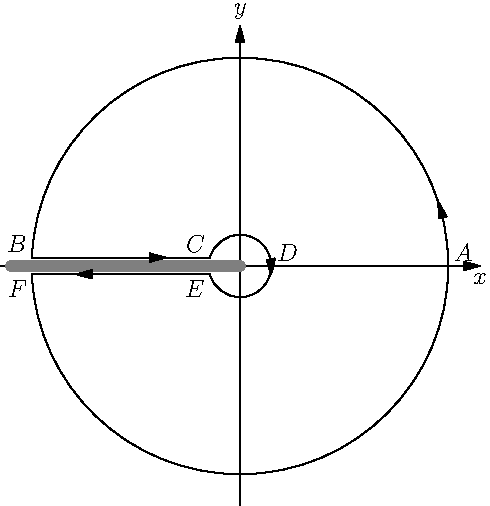
\includegraphics{graphics/contour_euler.pdf}
	\caption{Contour with a branch cut on the negative $x$-axis.}
\end{marginfigure}
%%%%%%%%%%%%%%%%%%%%%%%%%%%%%%%%%%%%

Using the Cauchy's theorem, we have
\[
   \int_C \frac{z^{x-1}}{1-z} dz = 2\pi i \, Res(z=1) = -2\pi i.
\]
Note that
\[
  \oint = \int_{FAB} + \int_{BC} + \int_{CDE} + \int_{EF},
\]
and it is easy to see that $\int_{FAB}=0$ from Jordan's lemma \ref{L:jordan}, 
and $\int_{CDE}=0$ because
\[
  \lim_{\epsilon\to 0} \left| \int_{CDE} \frac{z^{x-1}}{1-z} dz \right|
    \le \lim_{\epsilon\to 0} \int_{\pi}^{-\pi} 
      \frac{\epsilon^{x}}{|1-\epsilon e^{i\theta}|} d\theta 
    = 0.
\]
For line $BC$, let $z=w e^{i\pi}$, we get
\[
  \int_{BC} = \int_{\infty}^0 \frac{(we^{i\pi})^{x-1}}{1-we^{i\pi}} d(we^{i\pi})
     = -e^{i\pi x} \int_0^{\infty} \frac{w^{x-1}}{1+w} dw.
\]
For line $EF$, let $z=w e^{-i\pi}$, we get
\[
  \int_{EF} = \int_{\infty}^0 \frac{(we^{-i\pi})^{x-1}}{1-we^{-i\pi}} d(we^{-i\pi})
     = e^{-i\pi x} \int_0^{\infty} \frac{w^{x-1}}{1+w} dw.
\]
Hence we have
\[
  \int_{BC}+\int_{EF} 
    = (e^{-i\pi x}-e^{i\pi x}) \int_0^{\infty} \frac{w^{x-1}}{1+w} dw
    =-2\pi i,
\]
i.e.
\[
   \int_0^{\infty} \frac{w^{x-1}}{1+w} dw = \frac{\pi}{\sin(\pi x)},
\]
thus
\[
  \Gamma(1-x) \Gamma(x) = \frac{\pi}{\sin(\pi x)}.
 \]
\end{proof}


%%%%%%%%%%%%%%%%%%%%%%%%%%%%%%%%%%%%%%%%%%%%%%%%%%%%%%%%%%%%
\section{Bessel Function}

%%%%%%%%%%%%%%%%%%%%%%%%%%%%
\begin{definition} \label{D:bessel}
The modified Bessle function $J_{\nu}$ is defined by 
\footnote{Watson, A Treatise on the Theory of Bessel Functions, 3.7.(2), p77}
\begin{equation}
  J_{\nu}(z) = \sum_{m=0}^{\infty} \frac{(-)^m}{m! \Gamma(\nu+m+1)}
                \left(\frac{z}{2}\right)^{\nu+2m},
\end{equation}
\end{definition}

%%%%%%%%%%%%%%%%%%%%%%%%%%%%
\begin{definition} \label{D:bessel_mod}
The modified Bessle function $I_{\nu}$ is defined by 
\footnote{Watson, A Treatise on the Theory of Bessel Functions, 3.7.(2), p77}
\begin{equation}
  I_{\nu}(z) = \sum_{m=0}^{\infty} \frac{1}{m! \Gamma(\nu+m+1)}
                \left(\frac{z}{2}\right)^{\nu+2m},
\end{equation}
and $K_{\nu}$ is defined by
\begin{equation}
  K_{\nu}(z)=\frac{\pi}{2\sin{\pi\nu}} (I_{-\nu}(z) - I_{\nu}(z)).
\end{equation}
And $I_{\nu}(z)$ and $K_{\nu}(z)$ are independent solutions of the differential 
equation
\begin{equation}
  z^2 u''(z)+ z u'(z) - (z^2+\nu^2) u(z) = 0.
\end{equation}
\end{definition}

%%%%%%%%%%%%%%%%%%%%%%%%%%%%
\begin{proposition} \label{P:bessel_mod}
We have the following useful properties for the modified Bessel functions:
\begin{enumerate}
  \item[(1)] $K_{-\nu}(z) = K_{\nu}(z)$.
  \item[(2)] $I_{\nu}(z e^{in\pi}) = e^{in\nu\pi} I_{\nu}(z)$, and specifically
             $I_{\nu}(-z)=e^{i\nu\pi}I_{\nu}(z)$, here $n\in Z$.
  \item[(3)] $I_{\nu}(-x) K_{\nu}(-y) -I_{\nu}(x) K_{\nu}(y) =
  \frac{\pi}{2\sin(\pi\nu)} I_{\nu}(x) I_{\nu}(y) (e^{2i\nu\pi}-1)$.
\end{enumerate}
\end{proposition}
